\documentclass[tikz,border=10pt]{standalone}
\usepackage{amsmath}
\usepackage{tikz}
\usetikzlibrary{arrows.meta,calc,positioning}

\tikzset{
  signal/.style={->, line width=1.2pt, draw=black!80, >=Stealth},
  block/.style={draw=blue!70!black, line width=1.2pt, rectangle, minimum width=2.0cm, minimum height=1.0cm, fill=none},
  sum/.style={
    draw=green!55!black, line width=1.2pt, circle, minimum size=0.56cm, inner sep=0pt, fill=none,
    path picture={
      \draw[green!55!black, line width=0.9pt]
        (path picture bounding box.south west) -- (path picture bounding box.north east)
        (path picture bounding box.north west) -- (path picture bounding box.south east);
    }
  },
  tap/.style={draw=orange!85!black, line width=1.2pt, circle, minimum size=4.5pt, inner sep=0pt, fill=none},
  small/.style={font=\small}
}

\begin{document}
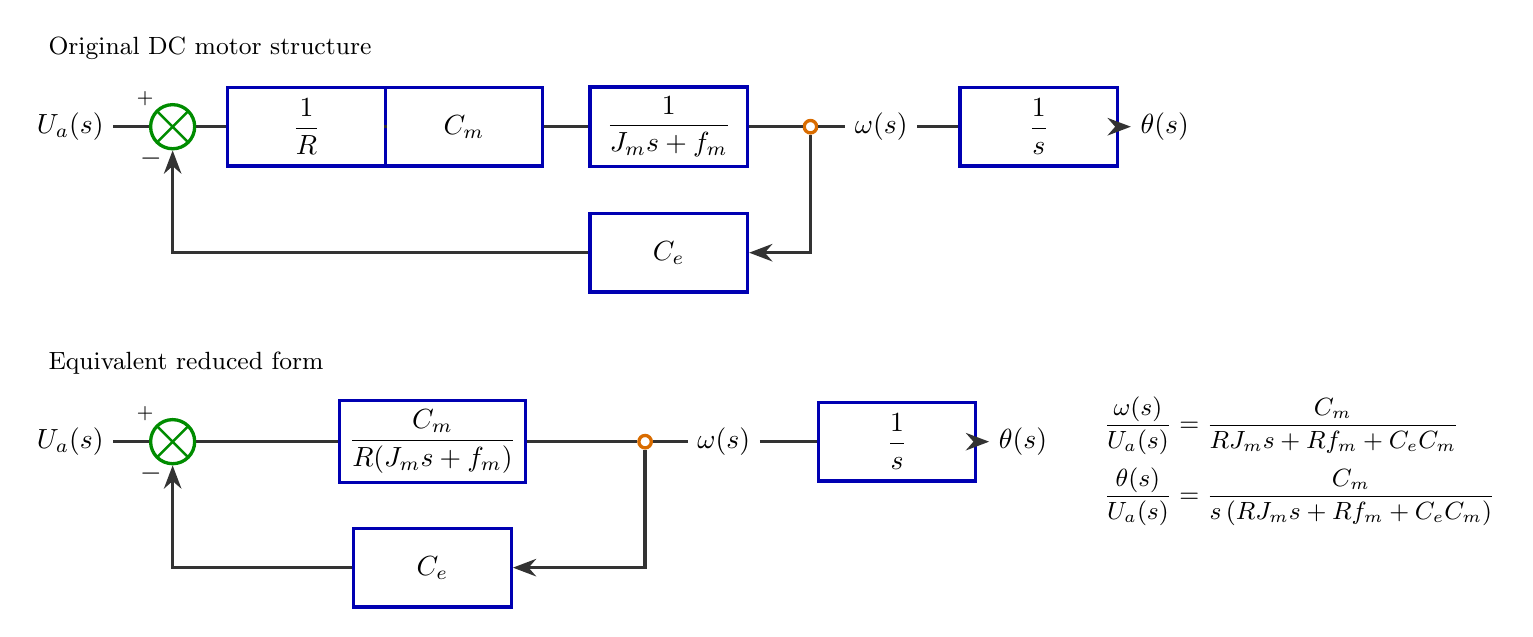
\begin{tikzpicture}
  \node[small, anchor=west] at (0,3.8) {Original DC motor structure};
  \node (ua) at (0.4,2.8) {$U_a(s)$};
  \node[sum] (sum1) at (1.7,2.8) {};
  \node[block] (r) at (3.4,2.8) {$\dfrac{1}{R}$};
  \node[block] (cm) at (5.4,2.8) {$C_m$};
  \node[block] (jm) at (8.0,2.8) {$\dfrac{1}{J_ms+f_m}$};
  \node[tap] (tpw) at (9.8,2.8) {};
  \node (w) at (10.7,2.8) {$\omega(s)$};
  \node[block] (intg) at (12.7,2.8) {$\dfrac{1}{s}$};
  \node (th) at (14.3,2.8) {$\theta(s)$};
  \node[block] (ce) at (8.0,1.2) {$C_e$};

  \draw[signal] (ua) -- (sum1) -- (r) -- (cm) -- (jm) -- (tpw) -- (w) -- (intg) -- (th);
  \draw[signal] (tpw) |- (ce);
  \draw[signal] (ce) -| node[pos=0.96, left] {$-$} (sum1.south);
  \node[font=\scriptsize] at ($(sum1)+(-0.35,0.35)$) {$+$};

  \node[small, anchor=west] at (0,-0.2) {Equivalent reduced form};
  \node (ua2) at (0.4,-1.2) {$U_a(s)$};
  \node[sum] (sum2) at (1.7,-1.2) {};
  \node[block] (g) at (5.0,-1.2) {$\dfrac{C_m}{R(J_ms+f_m)}$};
  \node[tap] (tp2) at (7.7,-1.2) {};
  \node (w2) at (8.7,-1.2) {$\omega(s)$};
  \node[block] (int2) at (10.9,-1.2) {$\dfrac{1}{s}$};
  \node (th2) at (12.5,-1.2) {$\theta(s)$};
  \node[block] (ce2) at (5.0,-2.8) {$C_e$};
  \draw[signal] (ua2) -- (sum2) -- (g) -- (tp2) -- (w2) -- (int2) -- (th2);
  \draw[signal] (tp2) |- (ce2);
  \draw[signal] (ce2) -| node[pos=0.96, left] {$-$} (sum2.south);
  \node[font=\scriptsize] at ($(sum2)+(-0.35,0.35)$) {$+$};

  \node[small, anchor=west] at (13.4,-1.0) {$\dfrac{\omega(s)}{U_a(s)}=\dfrac{C_m}{RJ_ms+Rf_m+C_eC_m}$};
  \node[small, anchor=west] at (13.4,-1.9) {$\dfrac{\theta(s)}{U_a(s)}=\dfrac{C_m}{s\left(RJ_ms+Rf_m+C_eC_m\right)}$};
\end{tikzpicture}
\end{document}
